% Options for packages loaded elsewhere
\PassOptionsToPackage{unicode}{hyperref}
\PassOptionsToPackage{hyphens}{url}
%
\documentclass[
]{article}
\title{Geopolitical Changes in the UNSC -- Is China's growing global
ambition reflected in its communication in the UNSC?}
\author{Erik Valentin Schulte\footnote{The project and the code is also
  available on:
  \url{https://github.com/eriksson396/Machine-Learning-Project}}}
\date{July 7th 2022}

\usepackage{amsmath,amssymb}
\usepackage{lmodern}
\usepackage{iftex}
\ifPDFTeX
  \usepackage[T1]{fontenc}
  \usepackage[utf8]{inputenc}
  \usepackage{textcomp} % provide euro and other symbols
\else % if luatex or xetex
  \usepackage{unicode-math}
  \defaultfontfeatures{Scale=MatchLowercase}
  \defaultfontfeatures[\rmfamily]{Ligatures=TeX,Scale=1}
\fi
% Use upquote if available, for straight quotes in verbatim environments
\IfFileExists{upquote.sty}{\usepackage{upquote}}{}
\IfFileExists{microtype.sty}{% use microtype if available
  \usepackage[]{microtype}
  \UseMicrotypeSet[protrusion]{basicmath} % disable protrusion for tt fonts
}{}
\makeatletter
\@ifundefined{KOMAClassName}{% if non-KOMA class
  \IfFileExists{parskip.sty}{%
    \usepackage{parskip}
  }{% else
    \setlength{\parindent}{0pt}
    \setlength{\parskip}{6pt plus 2pt minus 1pt}}
}{% if KOMA class
  \KOMAoptions{parskip=half}}
\makeatother
\usepackage{xcolor}
\IfFileExists{xurl.sty}{\usepackage{xurl}}{} % add URL line breaks if available
\IfFileExists{bookmark.sty}{\usepackage{bookmark}}{\usepackage{hyperref}}
\hypersetup{
  pdftitle={Geopolitical Changes in the UNSC -- Is China's growing global ambition reflected in its communication in the UNSC?},
  pdfauthor={Erik Valentin Schulte},
  hidelinks,
  pdfcreator={LaTeX via pandoc}}
\urlstyle{same} % disable monospaced font for URLs
\usepackage[margin=1in]{geometry}
\usepackage{color}
\usepackage{fancyvrb}
\newcommand{\VerbBar}{|}
\newcommand{\VERB}{\Verb[commandchars=\\\{\}]}
\DefineVerbatimEnvironment{Highlighting}{Verbatim}{commandchars=\\\{\}}
% Add ',fontsize=\small' for more characters per line
\usepackage{framed}
\definecolor{shadecolor}{RGB}{248,248,248}
\newenvironment{Shaded}{\begin{snugshade}}{\end{snugshade}}
\newcommand{\AlertTok}[1]{\textcolor[rgb]{0.94,0.16,0.16}{#1}}
\newcommand{\AnnotationTok}[1]{\textcolor[rgb]{0.56,0.35,0.01}{\textbf{\textit{#1}}}}
\newcommand{\AttributeTok}[1]{\textcolor[rgb]{0.77,0.63,0.00}{#1}}
\newcommand{\BaseNTok}[1]{\textcolor[rgb]{0.00,0.00,0.81}{#1}}
\newcommand{\BuiltInTok}[1]{#1}
\newcommand{\CharTok}[1]{\textcolor[rgb]{0.31,0.60,0.02}{#1}}
\newcommand{\CommentTok}[1]{\textcolor[rgb]{0.56,0.35,0.01}{\textit{#1}}}
\newcommand{\CommentVarTok}[1]{\textcolor[rgb]{0.56,0.35,0.01}{\textbf{\textit{#1}}}}
\newcommand{\ConstantTok}[1]{\textcolor[rgb]{0.00,0.00,0.00}{#1}}
\newcommand{\ControlFlowTok}[1]{\textcolor[rgb]{0.13,0.29,0.53}{\textbf{#1}}}
\newcommand{\DataTypeTok}[1]{\textcolor[rgb]{0.13,0.29,0.53}{#1}}
\newcommand{\DecValTok}[1]{\textcolor[rgb]{0.00,0.00,0.81}{#1}}
\newcommand{\DocumentationTok}[1]{\textcolor[rgb]{0.56,0.35,0.01}{\textbf{\textit{#1}}}}
\newcommand{\ErrorTok}[1]{\textcolor[rgb]{0.64,0.00,0.00}{\textbf{#1}}}
\newcommand{\ExtensionTok}[1]{#1}
\newcommand{\FloatTok}[1]{\textcolor[rgb]{0.00,0.00,0.81}{#1}}
\newcommand{\FunctionTok}[1]{\textcolor[rgb]{0.00,0.00,0.00}{#1}}
\newcommand{\ImportTok}[1]{#1}
\newcommand{\InformationTok}[1]{\textcolor[rgb]{0.56,0.35,0.01}{\textbf{\textit{#1}}}}
\newcommand{\KeywordTok}[1]{\textcolor[rgb]{0.13,0.29,0.53}{\textbf{#1}}}
\newcommand{\NormalTok}[1]{#1}
\newcommand{\OperatorTok}[1]{\textcolor[rgb]{0.81,0.36,0.00}{\textbf{#1}}}
\newcommand{\OtherTok}[1]{\textcolor[rgb]{0.56,0.35,0.01}{#1}}
\newcommand{\PreprocessorTok}[1]{\textcolor[rgb]{0.56,0.35,0.01}{\textit{#1}}}
\newcommand{\RegionMarkerTok}[1]{#1}
\newcommand{\SpecialCharTok}[1]{\textcolor[rgb]{0.00,0.00,0.00}{#1}}
\newcommand{\SpecialStringTok}[1]{\textcolor[rgb]{0.31,0.60,0.02}{#1}}
\newcommand{\StringTok}[1]{\textcolor[rgb]{0.31,0.60,0.02}{#1}}
\newcommand{\VariableTok}[1]{\textcolor[rgb]{0.00,0.00,0.00}{#1}}
\newcommand{\VerbatimStringTok}[1]{\textcolor[rgb]{0.31,0.60,0.02}{#1}}
\newcommand{\WarningTok}[1]{\textcolor[rgb]{0.56,0.35,0.01}{\textbf{\textit{#1}}}}
\usepackage{longtable,booktabs,array}
\usepackage{calc} % for calculating minipage widths
% Correct order of tables after \paragraph or \subparagraph
\usepackage{etoolbox}
\makeatletter
\patchcmd\longtable{\par}{\if@noskipsec\mbox{}\fi\par}{}{}
\makeatother
% Allow footnotes in longtable head/foot
\IfFileExists{footnotehyper.sty}{\usepackage{footnotehyper}}{\usepackage{footnote}}
\makesavenoteenv{longtable}
\usepackage{graphicx}
\makeatletter
\def\maxwidth{\ifdim\Gin@nat@width>\linewidth\linewidth\else\Gin@nat@width\fi}
\def\maxheight{\ifdim\Gin@nat@height>\textheight\textheight\else\Gin@nat@height\fi}
\makeatother
% Scale images if necessary, so that they will not overflow the page
% margins by default, and it is still possible to overwrite the defaults
% using explicit options in \includegraphics[width, height, ...]{}
\setkeys{Gin}{width=\maxwidth,height=\maxheight,keepaspectratio}
% Set default figure placement to htbp
\makeatletter
\def\fps@figure{htbp}
\makeatother
\setlength{\emergencystretch}{3em} % prevent overfull lines
\providecommand{\tightlist}{%
  \setlength{\itemsep}{0pt}\setlength{\parskip}{0pt}}
\setcounter{secnumdepth}{-\maxdimen} % remove section numbering
\newlength{\cslhangindent}
\setlength{\cslhangindent}{1.5em}
\newlength{\csllabelwidth}
\setlength{\csllabelwidth}{3em}
\newlength{\cslentryspacingunit} % times entry-spacing
\setlength{\cslentryspacingunit}{\parskip}
\newenvironment{CSLReferences}[2] % #1 hanging-ident, #2 entry spacing
 {% don't indent paragraphs
  \setlength{\parindent}{0pt}
  % turn on hanging indent if param 1 is 1
  \ifodd #1
  \let\oldpar\par
  \def\par{\hangindent=\cslhangindent\oldpar}
  \fi
  % set entry spacing
  \setlength{\parskip}{#2\cslentryspacingunit}
 }%
 {}
\usepackage{calc}
\newcommand{\CSLBlock}[1]{#1\hfill\break}
\newcommand{\CSLLeftMargin}[1]{\parbox[t]{\csllabelwidth}{#1}}
\newcommand{\CSLRightInline}[1]{\parbox[t]{\linewidth - \csllabelwidth}{#1}\break}
\newcommand{\CSLIndent}[1]{\hspace{\cslhangindent}#1}
\usepackage{booktabs}
\usepackage{longtable}
\usepackage{array}
\usepackage{multirow}
\usepackage{wrapfig}
\usepackage{float}
\usepackage{colortbl}
\usepackage{pdflscape}
\usepackage{tabu}
\usepackage{threeparttable}
\usepackage{threeparttablex}
\usepackage[normalem]{ulem}
\usepackage{makecell}
\usepackage{xcolor}
\ifLuaTeX
  \usepackage{selnolig}  % disable illegal ligatures
\fi

\begin{document}
\maketitle

\hypertarget{introduction}{%
\section{\texorpdfstring{Introduction
\label{Introduction}}{Introduction }}\label{introduction}}

Recently, the geopolitical architecture of the world is becoming more
and more challenged. Established institutions such as the United Nations
(UN) and its lower-tier institutions are shaken by international
disputes. One of the most apparent shifts is the ever-growing importance
of China in the international arena. This shift in power weights is also
reflected in China's international demeanor, diplomacy and
communication. The term ``wolf warrior diplomacy'' (Zhu 2020) became a
widespread synonym of this China's growing confidence and aggressive
representation of its policy objectives. Its claims in the congested and
strategically important South China Sea is one of the areas, where the
country's interests are represented vividly. Therefore, it would be
interesting if this development and shifts in policy objectives can also
be observed in China's official communication in the current
international institutions. China being a permanent member of the United
Nations Security Council (UNSC) and the importance of this body, makes
it an interesting case to study. The data by Schoenfeld et al. (2019)
are an ideal match for my study purposes. My first hypothesis is that
China's use of language became more demanding and direct given in light
of the wolf warrior diplomacy. Secondly, I would hypothesis that in
general China communicated more in this body and that topics directly
dealt with China's interests. Based on the theory of China's potential
shift in policy objectives in the UNSC, I now conduct the empirical
evaluation. For this purpose, I first describe the data preparation
process. Secondly, I conduct the actual computer assisted text analysis
which presents several measures and examines the hypotheses.

\hypertarget{link-between-machine-learning-and-text-analysis}{%
\section{Link between Machine Learning and Text
Analysis}\label{link-between-machine-learning-and-text-analysis}}

The data of the speeches of the Schoenfeld et al. (2019) data are
unstructured. Quantitative text analysis -- that is employed in this
paper -- is a machine learning (ML) technique that seeks to
automatically gain valuable insights from large amounts of unstructured
text data. The major challenge of quantitative text analysis is to take
the ambiguities of human language into account -- an issue that can only
be partially addressed in this paper. An example, is the negation word
``not,'' that may totally change the context in which certain words are
used. \newline My paper will solely focus on unsupervised machine
learning methods that are applied from Dotson (n.d.). In general,
quantitative text analysis is covered in parts of ML and Natural
Language Processing (NLP). I will cover text mining techniques such as
word frequency, text classification such as sentiment analysis and topic
modelling. Important challenges to apply ML to text is the complexity of
the analysis the conceptual difficulties (e.g.~humour/sarcasm in human
language) and taking into account cultural norms of communication
(Gavrilova 2020). For further reading on the link between text mining
and ML, I refer to Žižka, Dařena, and Svoboda (2019).

\hypertarget{data}{%
\section*{Data}\label{data}}
\addcontentsline{toc}{section}{Data}

First of all, I present all relevant data sources and explain essential
features to get a proper overview. Afterwards, I explain the process of
loading the data into R and how we process the raw text corpus, to
obtain meaningful results.\newline For our empirical analysis we use
three main data sources. The main data set comprises UN Security Council
debates between January 1995 and December 2020 and was downloaded from
Schoenfeld et al. (2019). The official meeting protocols are split into
distinct speeches. For every speech, metadata regarding the speaker, the
speaker's nation or affiliation, and the speaker's role in the meeting
is given. The topic of the meeting is also given. In total, the corpus
contains 82,165 speeches extracted from 5,748 meeting protocols. The
download file of Schoenfeld et al. (2019) also provides a code book with
the exact description of their workflow how to set-up the database as
well as a detailed variable description. \newline The data are split in
to a file containing all information about the UNSC meetings, one file
about the metadata of the speeches and one file containing the whole
text of the speeches. The other two data sources are word dictionaries
for the sentiment analysis. It is crucial for the sentiment analysis,
that the dictionaries are suitable for the specific context of analysis.
For example, a word list developed for sociology may not be a good fit
to analyze text data from for finance, and vice versa. The selection of
the right word lists is therefore of uttermost importance to get
meaningful and robust results Grimmer and Stewart (2013, 274--75).
Hence, I carefully choose only certain categories from the dictionaries
which are less prone to missclassification. Two wordlists namely Military
and Cooperation are from the most widely used standard dictionary, the
Harvard General Inquirer (see Hall (2019)). The other four wordlists:
Positive, Uncertainty, Strong Modal and Weak Modal are from
{``Documentation for the LoughranMcDonald\_MasterDictionary''}. Word
categories that were specially adapted to the financial context by
Loughran and McDonald (2011), such as the negative wordlist, are
neglected in my analysis.

\hypertarget{data-preparation}{%
\subsection{Data preparation}\label{data-preparation}}

In the next step, I import the speech data into R from the data folder
of my project file. To be able to process larger amounts of text, I need
special packages in R. These include the quanteda, quanteda.textplot and
quanteda.textstats. Other libraries like tidyverse, magrtittr, dyplr,
ggplot2, readtext, and kableExtra are used to manipulate the data and
plot it. We also set a seed, so that our results are reproducible.

\begin{Shaded}
\begin{Highlighting}[]
\CommentTok{\#load required packages}
\FunctionTok{library}\NormalTok{(tidyverse)}
\FunctionTok{library}\NormalTok{(readtext)}
\FunctionTok{library}\NormalTok{(quanteda)}
\FunctionTok{library}\NormalTok{(quanteda.textplots)}
\FunctionTok{library}\NormalTok{(quanteda.textstats)}
\FunctionTok{library}\NormalTok{(ggplot2)}
\FunctionTok{library}\NormalTok{(magrittr)}
\FunctionTok{library}\NormalTok{(gdata)}
\FunctionTok{library}\NormalTok{(kableExtra)}
\FunctionTok{library}\NormalTok{(tidytext)}
\FunctionTok{library}\NormalTok{(dplyr)}

\CommentTok{\#load the UN Security Council Debates dataset}
\FunctionTok{load}\NormalTok{(}\StringTok{"data/dataset.RData"}\NormalTok{)}
\FunctionTok{load}\NormalTok{(}\StringTok{"data/docs.RData"}\NormalTok{)}

\CommentTok{\#set a seed for reproducability}
\FunctionTok{set.seed}\NormalTok{(}\DecValTok{2333}\NormalTok{)}
\CommentTok{\# View data}
\CommentTok{\#head(meta\_meetings)}
\CommentTok{\#head(meta\_speeches)}
\end{Highlighting}
\end{Shaded}

I then rename the filename column of the data frame containing the
metadata of the speeches into doc\_id in order to have a common
identifier for merging with the actual text data from the speeches
(raw\_docs).

\begin{Shaded}
\begin{Highlighting}[]
\DocumentationTok{\#\#rename common column to merge the content of the speeches}
\NormalTok{meta\_speeches }\OtherTok{\textless{}{-}}\NormalTok{ meta\_speeches }\SpecialCharTok{\%\textgreater{}\%}
  \FunctionTok{rename}\NormalTok{(}\AttributeTok{doc\_id =}\NormalTok{ filename) }\SpecialCharTok{|}\ErrorTok{\textgreater{}} 
   \FunctionTok{filter}\NormalTok{(participanttype }\SpecialCharTok{!=} \StringTok{"The President"}\NormalTok{)}

\DocumentationTok{\#\# merge dataset raw with speeches}
\NormalTok{meta\_speeches }\OtherTok{\textless{}{-}} \FunctionTok{merge}\NormalTok{(meta\_speeches, raw\_docs, }\AttributeTok{by =} \StringTok{\textquotesingle{}doc\_id\textquotesingle{}}\NormalTok{)}
\end{Highlighting}
\end{Shaded}

In the next step I want to make a corpus from my data. The command
corpus comes from the quanteda package. Hence, the text column of the
meta\_speeces dataframe are now a corpus. I filter out speeches from the
president of the UNSC, as he or she mostly speaks on behalf of the
organization and not for their respective country. This reduces the
number of speeches by about 30,000 to 50,933.

\begin{Shaded}
\begin{Highlighting}[]
\CommentTok{\#as\_corpus\_frame(meta\_speeches$text, filter = NULL, row.names = NULL)}
\NormalTok{corp\_meta\_speeches }\OtherTok{\textless{}{-}} \FunctionTok{corpus}\NormalTok{(meta\_speeches, }\AttributeTok{text\_field =} \StringTok{"text"}\NormalTok{)}
\FunctionTok{summary}\NormalTok{(corp\_meta\_speeches, }\DecValTok{1}\NormalTok{)}
\end{Highlighting}
\end{Shaded}

\begin{verbatim}
## Corpus consisting of 50933 documents, showing 1 document:
## 
##                            Text Types Tokens Sentences speech
##  UNSC_1995_SPV.3487_spch002.txt   575   1746        45      2
##                 country      speaker participanttype role_in_un  spv
##  Bosnia And Herzegovina Mr. Sacirbey           Guest            3487
##            basename
##  UNSC_1995_SPV.3487
##                                                               topic
##  Federal Republic of Yugoslavia (Serbia and Montenegro) — Sanctions
##             date year month day types tokens sentences
##  12 January 1995 1995     1  12   575   1746        45
##                                                    topic2
##  Items relating to the situation in the former Yugoslavia
##                subtopic agenda_item1      agenda_item2           agenda_item3
##  Bosnia and Herzegovina       Europe Former Yugoslavia Bosnia and Herzegovina
##  decision
##      <NA>
\end{verbatim}

\begin{Shaded}
\begin{Highlighting}[]
\NormalTok{corp\_meta\_speeches }\OtherTok{\textless{}{-}} \FunctionTok{corpus\_subset}\NormalTok{(corp\_meta\_speeches, participanttype }\SpecialCharTok{!=} \StringTok{"The President"}\NormalTok{)}
\end{Highlighting}
\end{Shaded}

I also create a unique corpus just for the speeches held by China. I do
this using the corpus\_subset command from my previously defined corpus.
I also take a subset of the meta\_speeches dataframe with only the
speeches from China. In total there are 3564 speeches by China in the
dataframe, a total share of 3.82\% of all speeches. So there appear to
be 1619 speeches from China as participant type president. So, the
speeches where china speaks on behalf of the president are excluded.

\begin{Shaded}
\begin{Highlighting}[]
\CommentTok{\#How do I assign the speeches to the columns (now the speeches are in the same order as in the document, but not tied to the countries)}

\NormalTok{corp\_China }\OtherTok{\textless{}{-}} \FunctionTok{corpus\_subset}\NormalTok{(corp\_meta\_speeches, country }\SpecialCharTok{==} \StringTok{"China"}\NormalTok{)}
\NormalTok{Chinaspeeches }\OtherTok{\textless{}{-}} \FunctionTok{subset.data.frame}\NormalTok{(meta\_speeches, country }\SpecialCharTok{==} \StringTok{"China"}\NormalTok{)}
\NormalTok{share\_CHN\_speeches }\OtherTok{\textless{}{-}} \DecValTok{1945}\SpecialCharTok{/}\DecValTok{50933}
\CommentTok{\#*}
\CommentTok{\#only creates value, which I mention in the text.}

\DocumentationTok{\#\# access to document level variables of the China corpus}
\FunctionTok{head}\NormalTok{(}\FunctionTok{docvars}\NormalTok{(corp\_China))}
\end{Highlighting}
\end{Shaded}

\begin{verbatim}
##   speech country          speaker participanttype role_in_un             spv
## 1     30   China Mr. Wang Xuexian       Mentioned                       3487
## 2      4   China Mr. Wang Xuexian       Mentioned                       3489
## 3      7   China Mr. Wang Xuexian       Mentioned                       3492
## 4     11   China  Mr. Li Zhaoxing       Mentioned                       3494
## 5     13   China  Mr. Li Zhaoxing       Mentioned                       3496
## 6     16   China Mr. Wang Xuexian       Mentioned            3499Resumption1
##                        basename
## 1            UNSC_1995_SPV.3487
## 2            UNSC_1995_SPV.3489
## 3            UNSC_1995_SPV.3492
## 4            UNSC_1995_SPV.3494
## 5            UNSC_1995_SPV.3496
## 6 UNSC_1995_SPV.3499Resumption1
##                                                                topic
## 1 Federal Republic of Yugoslavia (Serbia and Montenegro) — Sanctions
## 2                                                            Liberia
## 3                                                   Agenda for Peace
## 4                                                         Mozambique
## 5                                                              Haiti
## 6                                                             Angola
##              date year month day types tokens sentences
## 1 12 January 1995 1995     1  12   287    707        22
## 2 13 January 1995 1995     1  13   202    432        16
## 3 18 January 1995 1995     1  18   670   1948        69
## 4 27 January 1995 1995     1  27   261    553        18
## 5 30 January 1995 1995     1  30   197    373        14
## 6 8 February 1995 1995     2   8   358    902        28
##                                                     topic2
## 1 Items relating to the situation in the former Yugoslavia
## 2                                 The situation in Liberia
## 3                    Items relating to an Agenda for Peace
## 4                              The situation in Mozambique
## 5                            The question concerning Haiti
## 6                                  The situation in Angola
##                                subtopic agenda_item1      agenda_item2
## 1                Bosnia and Herzegovina       Europe Former Yugoslavia
## 2              The situation in Liberia       Africa           Liberia
## 3 Items relating to an Agenda for Peace     Thematic  Agenda for peace
## 4           The situation in Mozambique       Africa        Mozambique
## 5         The question concerning Haiti     Americas             Haiti
## 6               The situation in Angola       Africa            Angola
##             agenda_item3 decision
## 1 Bosnia and Herzegovina     <NA>
## 2                Liberia     <NA>
## 3               Thematic     <NA>
## 4             Mozambique     <NA>
## 5                  Haiti     <NA>
## 6                 Angola     <NA>
\end{verbatim}

\begin{Shaded}
\begin{Highlighting}[]
\DocumentationTok{\#\#extract them the document level variables}
\CommentTok{\#docvars(corp\_China, field = "speaker")}

\CommentTok{\#corp\_China$year}

\DocumentationTok{\#\#create new variables (does not work yet)}
\CommentTok{\#corp\_China$avg\_speech\_length \textless{}{-} (mean(corp\_China$sentences))}
\CommentTok{\#avg\_speech\_length}
\end{Highlighting}
\end{Shaded}

As a next step, I separate the whole speeches into sentences in tidy
format. One column for every sentence of a speech. For that I use the
unnest\_tokens function from the tidytext package. This lets the the
number of observations grow to 1,767,696 million. The problem here is
that now after every salutation like ``Mr.'' so after every point the
function creates a new sentence. When we create a dataframe for every
word as an observation, the number of observation grows to 43,534,652
million. Therefore, we must clean the data further before using them for
analysis.

\begin{Shaded}
\begin{Highlighting}[]
\DocumentationTok{\#\#separates by default into words all speeches from raw docs (here by sentences) variable after tokens}
\NormalTok{tidy\_raw\_sentences }\OtherTok{\textless{}{-}}\NormalTok{ meta\_speeches }\SpecialCharTok{\%\textgreater{}\%}
  \FunctionTok{unnest\_tokens}\NormalTok{(sentences\_content, text, }\AttributeTok{token =} \StringTok{"sentences"}\NormalTok{ )}

\DocumentationTok{\#\#separate into words a new variable each word per speech (gives us 47,4 Mio obs.)}
\NormalTok{tidy\_raw\_words }\OtherTok{\textless{}{-}}\NormalTok{ meta\_speeches }\SpecialCharTok{|}\ErrorTok{\textgreater{}} 
    \FunctionTok{unnest\_tokens}\NormalTok{(word, text)}
\end{Highlighting}
\end{Shaded}

The tidytext package also come with a list of stop words -- words that
are not meaningful and that we want to exclude from the analysis. The
stop words list contains 1149 words. Our data frame reduces to
19,623,316 million observations -- by more than a half. This allows me
to start with a first analysis. I can plot the most frequent words used
in the speeches of the UNSC. For that, I plot the most common words that
were used more than 80,000 times in total. The threshold of 65,000 is
subjectively chosen and is based on the graphical aesthetics.

\begin{Shaded}
\begin{Highlighting}[]
\DocumentationTok{\#\#remove redundant words (reduces from 47,6 Mio words to 21,4 Mio words)}
\FunctionTok{data}\NormalTok{(stop\_words)  }\DocumentationTok{\#\#this comes with a package (a list of unuseful words)}

\NormalTok{tidy\_raw\_words }\OtherTok{\textless{}{-}}\NormalTok{ tidy\_raw\_words }\SpecialCharTok{\%\textgreater{}\%}
  \FunctionTok{anti\_join}\NormalTok{(stop\_words)}

\DocumentationTok{\#\#count words, after redundant words were removed (only meaningful words)}
\CommentTok{\# tidy\_raw\_words \%\textgreater{}\%}
\CommentTok{\#   count(word, sort = TRUE)}
\end{Highlighting}
\end{Shaded}

\hypertarget{a-first-visual-inspection-of-the-most-commonly-used-words}{%
\section{A first visual inspection of the most commonly used
words}\label{a-first-visual-inspection-of-the-most-commonly-used-words}}

We can see from the graph that council, security and united are the most
frequently used words. This gives are first overview of the most used
words.

\includegraphics{Final-Output,-ML_files/figure-latex/unnamed-chunk-7-1.pdf}
I also plot the 40 most common words from the UNSC in a wordcloud.

\begin{Shaded}
\begin{Highlighting}[]
\CommentTok{\# Load the wordcloud package}
\FunctionTok{library}\NormalTok{(wordcloud)}

\CommentTok{\# Compute word counts and assign to word\_counts}
\NormalTok{word\_counts\_UNSC }\OtherTok{\textless{}{-}}\NormalTok{ tidy\_raw\_words }\SpecialCharTok{\%\textgreater{}\%} 
  \FunctionTok{count}\NormalTok{(word)}

\FunctionTok{wordcloud}\NormalTok{(}
  \CommentTok{\# Assign the word column to words}
  \AttributeTok{word =}\NormalTok{ word\_counts\_UNSC}\SpecialCharTok{$}\NormalTok{word, }
  \CommentTok{\# Assign the count column to freq}
  \AttributeTok{freq =}\NormalTok{word\_counts\_UNSC}\SpecialCharTok{$}\NormalTok{n,}
  \AttributeTok{scale=}\FunctionTok{c}\NormalTok{(}\DecValTok{2}\NormalTok{,.}\DecValTok{4}\NormalTok{),}
  \AttributeTok{max.words =} \DecValTok{40}\NormalTok{,}
  \AttributeTok{colors =} \StringTok{"blue"}
\NormalTok{)}
\end{Highlighting}
\end{Shaded}

\includegraphics{Final-Output,-ML_files/figure-latex/unnamed-chunk-8-1.pdf}
I then apply the same analysis for the data frame from the Chinese
speeches.

\includegraphics{Final-Output,-ML_files/figure-latex/unnamed-chunk-10-1.pdf}

Additionally, I visualize the 40 most common words in a wordcloud using
the wordcloud package.

\begin{Shaded}
\begin{Highlighting}[]
\CommentTok{\# Load the wordcloud package}
\FunctionTok{library}\NormalTok{(wordcloud)}

\CommentTok{\# Compute word counts and assign to word\_counts}
\NormalTok{word\_counts\_CHN }\OtherTok{\textless{}{-}}\NormalTok{ tidy\_raw\_words\_CHN }\SpecialCharTok{\%\textgreater{}\%} 
  \FunctionTok{count}\NormalTok{(word)}

\FunctionTok{wordcloud}\NormalTok{(}
  \CommentTok{\# Assign the word column to words}
  \AttributeTok{word =}\NormalTok{ word\_counts\_CHN}\SpecialCharTok{$}\NormalTok{word, }
  \CommentTok{\# Assign the count column to freq}
  \AttributeTok{freq =}\NormalTok{word\_counts\_CHN}\SpecialCharTok{$}\NormalTok{n,}
  \AttributeTok{scale=}\FunctionTok{c}\NormalTok{(}\DecValTok{2}\NormalTok{,.}\DecValTok{4}\NormalTok{),}
  \AttributeTok{max.words =} \DecValTok{40}\NormalTok{,}
  \AttributeTok{colors =} \StringTok{"red"}
\NormalTok{)}
\end{Highlighting}
\end{Shaded}

\includegraphics{Final-Output,-ML_files/figure-latex/unnamed-chunk-11-1.pdf}
A central question in text mining and natural language processing is how
to quantify what a document is about. One measure of how important a
word may be is its term frequency (tf), how frequently a word occurs in
a document.

\hypertarget{frequency-terms}{%
\section{Frequency terms}\label{frequency-terms}}

Next, I calculate frequency terms. The function get\_freqs creates a
list of the frequency of terms that appear in each speech. The function
takes the respective corpus as an input and returns the frequencies in
the form of a data frame. In the first step, it creates tokens from the
text documents. Tokens are a sequence of elementary lexical components,
in our case words. Punctuation, separators and stop words like ``he,''
``do,'' or ``if'' are excluded as they have no meaning for the content
and therefore represent no real added value for the analysis. The dfm()
function is then applied to the tokens to create the document feature
matrix (dfm). As the dfm is a very sparse matrix containing the
documents as rows and the terms as columns, I aggregate the data over
all documents and sort the frequency of the terms in a descending order
using the textstat\_frequency() command. In addition, a special feature
of the get\_freqs function is the weighting parameter, which is set to
FALSE per default. If it is being activated the frequencies are weighted
according to the term-frequency inverse document frequency (tf.idf)
weighting scheme. This measures how important a word is to a document
compared with a corpus of other documents, e.g.~one short story in a
collection of short stories.

\(idf(\text{term}) = \ln{\left(\frac{n_{\text{documents}}}{n_{\text{documents containing term}}}\right)}\)

In the end we apply the get\_dfm function to the two corpora and save
the result in the variable freqs\_all and freqs\_CHN respectively.

\begin{Shaded}
\begin{Highlighting}[]
\CommentTok{\#calculate the frequency of terms that appear in each speech. It also creates a document feature matrix.}
\CommentTok{\#frequency of each word in the corpus}
\CommentTok{\# function takes the respective corpus as an input and returns the frequencies in the form of a data frame}


\NormalTok{get\_freqs }\OtherTok{\textless{}{-}} \ControlFlowTok{function}\NormalTok{(corp\_meta\_speeches, }\AttributeTok{weighting =} \ConstantTok{TRUE}\NormalTok{)\{}
\NormalTok{tokens }\OtherTok{\textless{}{-}} \FunctionTok{tokens}\NormalTok{(corp\_meta\_speeches, }\AttributeTok{remove\_punct =}\NormalTok{ T, }\AttributeTok{remove\_separators =}\NormalTok{ T, }\AttributeTok{include\_docvars =}\NormalTok{ T)}
\NormalTok{tokens }\OtherTok{\textless{}{-}} \FunctionTok{tokens\_remove}\NormalTok{(tokens, }\FunctionTok{stopwords}\NormalTok{(}\StringTok{"en"}\NormalTok{))}
\NormalTok{dfm }\OtherTok{\textless{}{-}}\NormalTok{ tokens }\SpecialCharTok{\%\textgreater{}\%} \FunctionTok{dfm}\NormalTok{()}
\NormalTok{freqs }\OtherTok{\textless{}{-}} \FunctionTok{textstat\_frequency}\NormalTok{(dfm)}

\ControlFlowTok{if}\NormalTok{(weighting }\SpecialCharTok{==} \ConstantTok{TRUE}\NormalTok{)\{}
\NormalTok{freqs}\SpecialCharTok{$}\NormalTok{term\_frequency }\OtherTok{\textless{}{-}}\NormalTok{ freqs}\SpecialCharTok{$}\NormalTok{frequency }\SpecialCharTok{/} \FunctionTok{sum}\NormalTok{(freqs}\SpecialCharTok{$}\NormalTok{frequency)}
\NormalTok{freqs}\SpecialCharTok{$}\NormalTok{inverse\_doc\_freq }\OtherTok{\textless{}{-}} \FunctionTok{log10}\NormalTok{( }\FunctionTok{length}\NormalTok{(corp\_meta\_speeches) }\SpecialCharTok{/}\NormalTok{ freqs}\SpecialCharTok{$}\NormalTok{docfreq )}
\NormalTok{freqs}\SpecialCharTok{$}\NormalTok{frequency }\OtherTok{\textless{}{-}}\NormalTok{ freqs}\SpecialCharTok{$}\NormalTok{term\_frequency}\SpecialCharTok{*}\NormalTok{freqs}\SpecialCharTok{$}\NormalTok{inverse\_doc\_freq}
\NormalTok{\}}
\FunctionTok{return}\NormalTok{(freqs)}

\NormalTok{\}}

\NormalTok{freqs\_CHN }\OtherTok{\textless{}{-}} \FunctionTok{get\_freqs}\NormalTok{(corp\_China,}\AttributeTok{weighting=}\ConstantTok{TRUE}\NormalTok{)}
\NormalTok{freqs\_all }\OtherTok{\textless{}{-}} \FunctionTok{get\_freqs}\NormalTok{(corp\_meta\_speeches,}\AttributeTok{weighting =} \ConstantTok{TRUE}\NormalTok{)}

\CommentTok{\#Mr. und Mrs. is still inside, maybe you can research something on the gender of the diplomats}
\end{Highlighting}
\end{Shaded}

We then get a new dataframe with each word, the frequency (percentage
share of appearance of all words), the rank based on the frequency, the
total document frequency of the words, the term\_frequency and the
inverse\_term\_frequency.

Creating a dataframe which counts every word and shows that we have
13494 unique words in the dataframe used by China after deleting the
stopwords.

\begin{Shaded}
\begin{Highlighting}[]
\NormalTok{speech\_words\_CHN }\OtherTok{\textless{}{-}}\NormalTok{ tidy\_raw\_words\_CHN }\SpecialCharTok{\%\textgreater{}\%}
 \CommentTok{\# unnest\_tokens(word, text) \%\textgreater{}\%}
  \FunctionTok{count}\NormalTok{(word, }\AttributeTok{sort =} \ConstantTok{TRUE}\NormalTok{) }\SpecialCharTok{|}\ErrorTok{\textgreater{}} 
    \FunctionTok{mutate}\NormalTok{(}\AttributeTok{total =} \FunctionTok{sum}\NormalTok{(n))}

\NormalTok{speech\_words\_CHN\_per\_speech }\OtherTok{\textless{}{-}}\NormalTok{ tidy\_raw\_words\_CHN }\SpecialCharTok{\%\textgreater{}\%}
 \CommentTok{\# unnest\_tokens(word, text) \%\textgreater{}\%}
  \FunctionTok{count}\NormalTok{(speech, word, }\AttributeTok{sort =} \ConstantTok{TRUE}\NormalTok{) }\SpecialCharTok{|}\ErrorTok{\textgreater{}} \CommentTok{\#mit speech dann ist es per speech sortiert....}
    \FunctionTok{mutate}\NormalTok{(}\AttributeTok{total =} \FunctionTok{sum}\NormalTok{(n))}
\end{Highlighting}
\end{Shaded}

\hypertarget{visualizing-term-frequency-in-chinas-speeches}{%
\subsection{Visualizing term frequency in China's
speeches}\label{visualizing-term-frequency-in-chinas-speeches}}

The graph shows the number of times a word appears in the speeches
divided by the total number of terms (words) in the speeches. There are
very long tails to the right for the Chinese speeches (those extremely
rare words!) that I do not include in the plot. Many words occur rarely
and few words occur frequently.

\begin{Shaded}
\begin{Highlighting}[]
\FunctionTok{ggplot}\NormalTok{(speech\_words\_CHN, }\FunctionTok{aes}\NormalTok{(n}\SpecialCharTok{/}\NormalTok{total)) }\SpecialCharTok{+}
  \FunctionTok{geom\_histogram}\NormalTok{(}\AttributeTok{show.legend =} \ConstantTok{FALSE}\NormalTok{) }\SpecialCharTok{+}
  \FunctionTok{xlim}\NormalTok{(}\ConstantTok{NA}\NormalTok{, }\FloatTok{0.0009}\NormalTok{) }\SpecialCharTok{+}
    \FunctionTok{labs}\NormalTok{(}
        \AttributeTok{title =} \StringTok{"Term frequency distribtion in China\textquotesingle{}s speeches"}\NormalTok{,}
        \AttributeTok{subtitle =} \StringTok{"Distribution of frequency of words divided by total words"}
\NormalTok{    )}
\end{Highlighting}
\end{Shaded}

\begin{verbatim}
## `stat_bin()` using `bins = 30`. Pick better value with `binwidth`.
\end{verbatim}

\begin{verbatim}
## Warning: Removed 195 rows containing non-finite values (stat_bin).
\end{verbatim}

\begin{verbatim}
## Warning: Removed 1 rows containing missing values (geom_bar).
\end{verbatim}

\includegraphics{Final-Output,-ML_files/figure-latex/unnamed-chunk-14-1.pdf}

\begin{Shaded}
\begin{Highlighting}[]
\CommentTok{\#  facet\_wrap(\textasciitilde{}book, ncol = 2, scales = "free\_y")}
\end{Highlighting}
\end{Shaded}

The distribution we can see here is common in language. These
long-tailed distributions are very common in natural language (like
books, a lot of text from a website, or spoken words). Hence, the
relationship between the frequency that a word is used and its rank has
been the subject of study. A famous version of this relationship is
called Zipf's law, after George Zipf, a 20th century American linguist.
Zipf's law states that the frequency that a word appears is inversely
proportional to its rank Silge and Robinson (2017).

\begin{Shaded}
\begin{Highlighting}[]
\NormalTok{freq\_by\_rank\_CHN }\OtherTok{\textless{}{-}}\NormalTok{ speech\_words\_CHN }\SpecialCharTok{\%\textgreater{}\%} 
  \FunctionTok{mutate}\NormalTok{(}\AttributeTok{rank =} \FunctionTok{row\_number}\NormalTok{(), }
         \StringTok{\textasciigrave{}}\AttributeTok{term frequency}\StringTok{\textasciigrave{}} \OtherTok{=}\NormalTok{ n}\SpecialCharTok{/}\NormalTok{total) }\SpecialCharTok{\%\textgreater{}\%}
  \FunctionTok{ungroup}\NormalTok{()}

\FunctionTok{head}\NormalTok{(freq\_by\_rank\_CHN)}
\end{Highlighting}
\end{Shaded}

\begin{verbatim}
##            word    n  total rank term frequency
## 1         china 9476 522480    1     0.01813658
## 2 international 8150 522480    2     0.01559868
## 3      security 7414 522480    3     0.01419002
## 4         peace 7095 522480    4     0.01357947
## 5        united 5980 522480    5     0.01144541
## 6       nations 5550 522480    6     0.01062242
\end{verbatim}

The rank column here tells us the rank of each word within the frequency
table; the table was already ordered by n so we could use row\_number()
to find the rank. Then, we can calculate the term frequency in the same
way we did before. Zipf's law is often visualized by plotting rank on
the x-axis and term frequency on the y-axis, on logarithmic scales.
Plotting this way, an inversely proportional relationship will have a
constant, negative slope.

\hypertarget{zipfs-law}{%
\subsubsection{Zipf's law}\label{zipfs-law}}

\begin{Shaded}
\begin{Highlighting}[]
\NormalTok{freq\_by\_rank\_CHN }\SpecialCharTok{\%\textgreater{}\%} 
  \FunctionTok{ggplot}\NormalTok{(}\FunctionTok{aes}\NormalTok{(rank, }\StringTok{\textasciigrave{}}\AttributeTok{term frequency}\StringTok{\textasciigrave{}}\NormalTok{)) }\SpecialCharTok{+} 
  \FunctionTok{geom\_line}\NormalTok{(}\AttributeTok{size =} \FloatTok{1.1}\NormalTok{, }\AttributeTok{alpha =} \FloatTok{0.8}\NormalTok{, }\AttributeTok{show.legend =} \ConstantTok{FALSE}\NormalTok{) }\SpecialCharTok{+} 
  \FunctionTok{scale\_x\_log10}\NormalTok{() }\SpecialCharTok{+}
  \FunctionTok{scale\_y\_log10}\NormalTok{() }\SpecialCharTok{+}
    \FunctionTok{labs}\NormalTok{(}
        \AttributeTok{title =} \StringTok{"Zipf\textquotesingle{}s Law for China\textquotesingle{}s speeches in the UNSC"}
\NormalTok{    )}
\end{Highlighting}
\end{Shaded}

\includegraphics{Final-Output,-ML_files/figure-latex/unnamed-chunk-16-1.pdf}

\begin{Shaded}
\begin{Highlighting}[]
\CommentTok{\#How could I plot the same for all speeches?}
\end{Highlighting}
\end{Shaded}

Notice that the Zipf's law figure is in log-log coordinates. We see that
the relationship between rank and frequency does have a negative slope.
It is not quite constant, though; perhaps we could view this as a broken
power law. Let's see what the exponent of the power law is for the
middle section (between ranks 10 and 500) of the rank range (Silge and
Robinson 2017).

\begin{Shaded}
\begin{Highlighting}[]
\NormalTok{rank\_subset }\OtherTok{\textless{}{-}}\NormalTok{ freq\_by\_rank\_CHN }\SpecialCharTok{\%\textgreater{}\%} 
  \FunctionTok{filter}\NormalTok{(rank }\SpecialCharTok{\textless{}} \DecValTok{500}\NormalTok{,}
\NormalTok{         rank }\SpecialCharTok{\textgreater{}} \DecValTok{10}\NormalTok{)}

\FunctionTok{lm}\NormalTok{(}\FunctionTok{log10}\NormalTok{(}\StringTok{\textasciigrave{}}\AttributeTok{term frequency}\StringTok{\textasciigrave{}}\NormalTok{) }\SpecialCharTok{\textasciitilde{}} \FunctionTok{log10}\NormalTok{(rank), }\AttributeTok{data =}\NormalTok{ rank\_subset)}
\end{Highlighting}
\end{Shaded}

\begin{verbatim}
## 
## Call:
## lm(formula = log10(`term frequency`) ~ log10(rank), data = rank_subset)
## 
## Coefficients:
## (Intercept)  log10(rank)  
##     -1.1924      -0.8191
\end{verbatim}

Classi versions of Zipf's law:
\(\text{frequency} \propto \frac{1}{\text{rank}}\)

\begin{Shaded}
\begin{Highlighting}[]
\NormalTok{freq\_by\_rank\_CHN }\SpecialCharTok{\%\textgreater{}\%} 
  \FunctionTok{ggplot}\NormalTok{(}\FunctionTok{aes}\NormalTok{(rank, }\StringTok{\textasciigrave{}}\AttributeTok{term frequency}\StringTok{\textasciigrave{}}\NormalTok{)) }\SpecialCharTok{+} 
  \FunctionTok{geom\_abline}\NormalTok{(}\AttributeTok{intercept =} \SpecialCharTok{{-}}\FloatTok{1.19}\NormalTok{, }\AttributeTok{slope =} \SpecialCharTok{{-}}\FloatTok{0.81}\NormalTok{, }\CommentTok{\#take these numbers from the regression above}
              \AttributeTok{color =} \StringTok{"red"}\NormalTok{, }\AttributeTok{linetype =} \DecValTok{4}\NormalTok{) }\SpecialCharTok{+}
  \FunctionTok{geom\_line}\NormalTok{(}\AttributeTok{size =} \FloatTok{1.1}\NormalTok{, }\AttributeTok{alpha =} \FloatTok{0.8}\NormalTok{, }\AttributeTok{show.legend =} \ConstantTok{FALSE}\NormalTok{) }\SpecialCharTok{+} 
  \FunctionTok{scale\_x\_log10}\NormalTok{() }\SpecialCharTok{+}
  \FunctionTok{scale\_y\_log10}\NormalTok{() }\SpecialCharTok{+}
    \FunctionTok{labs}\NormalTok{(}
        \AttributeTok{title =} \StringTok{"Fitting an exponent for Zipf\textquotesingle{}s Law with China\textquotesingle{}s speeches in the UNSC"}\NormalTok{)}
\end{Highlighting}
\end{Shaded}

\includegraphics{Final-Output,-ML_files/figure-latex/unnamed-chunk-18-1.pdf}
We have found a result close to the classic version of Zipf's law for
the corpus of China's UNSC speeches. The deviations we see here at high
rank are not uncommon for many kinds of language; a corpus of language
often contains fewer rare words than predicted by a single power law.
The deviations at low rank are more less unusual compared to the
deviations from the fitted line at high rank. China uses a lower
percentage of uncommon words than many collections of language, which
may indicate the complexity of the diplomatic language.

\hypertarget{the-bind_tf_idf-function}{%
\subsection{The bind\_tf\_idf()
function}\label{the-bind_tf_idf-function}}

The idea of tf-idf is to find the important words for the content of
each document by decreasing the weight for commonly used words and
increasing the weight for words that are not used very much in a
collection or corpus of documents, in this case, the speeches by China
in the UNSC. Calculating tf-idf attempts to find the words that are
important (i.e., common) in a text, but not too common.

The bind\_tf\_idf() function in the tidytext package takes a tidy text
dataset as input. One column (word here) contains the terms/tokens, one
column contains the documents (speech in this case), and the last
necessary column contains the counts, how many times each speech
contains each term (n in this example). I create a new dataframe for
this, as the bind\_tf\_idf function requires a document entry (speeches
in my case).

\begin{Shaded}
\begin{Highlighting}[]
\NormalTok{CHN\_tf\_idf }\OtherTok{\textless{}{-}}\NormalTok{ speech\_words\_CHN\_per\_speech }\SpecialCharTok{\%\textgreater{}\%}  \CommentTok{\#89955 variables...}
  \FunctionTok{bind\_tf\_idf}\NormalTok{(word, speech, n)}

\FunctionTok{head}\NormalTok{(CHN\_tf\_idf)}
\end{Highlighting}
\end{Shaded}

\begin{verbatim}
##   speech          word   n  total         tf        idf       tf_idf
## 1     12         china 689 522480 0.02115054 0.00000000 0.0000000000
## 2     11         china 658 522480 0.01835938 0.00000000 0.0000000000
## 3     13         china 652 522480 0.01825257 0.00000000 0.0000000000
## 4     14         china 597 522480 0.01729182 0.00000000 0.0000000000
## 5     10         china 581 522480 0.01923586 0.00000000 0.0000000000
## 6     13 international 576 522480 0.01612497 0.02247286 0.0003623741
\end{verbatim}

The idf and thus tf-idf are zero for these most common words (China).
Unsurprisingly, the word China appears very often in the speeches of
China, so the idf-term (which will then be the natural log of 1) is
zero. The inverse document frequency (and thus tf-idf) is close to zero
for words that occur in many of the speeches in a collection. This is,
in fact, the procedure how this approach decreases the weight for common
words. The inverse document frequency will be a higher number for words
that occur in fewer speeches.

Here we see important words that are in fact important in these
respective speeches. None of them occurs in all of speeches. But they
are important, characteristic words for each speech within the corpus of
the UNSC speeches by China. We can see that one speech (speech 129) most
likely talked about the still ongoing territorial disputes in the South
China Sea, as nansha, islands, and sea were important words in that
speech.

\begin{Shaded}
\begin{Highlighting}[]
\CommentTok{\#make this example reproducible}
\FunctionTok{set.seed}\NormalTok{(}\DecValTok{1}\NormalTok{)}

\CommentTok{\#define data}
\NormalTok{high\_tf\_idf\_CHN }\OtherTok{\textless{}{-}} \FunctionTok{data.frame}\NormalTok{(}\AttributeTok{speech=}\FunctionTok{c}\NormalTok{(}\StringTok{\textquotesingle{}110\textquotesingle{}}\NormalTok{, }\StringTok{"129"}\NormalTok{, }\StringTok{\textquotesingle{}129\textquotesingle{}}\NormalTok{, }\StringTok{\textquotesingle{}51\textquotesingle{}}\NormalTok{, }\StringTok{"129"}\NormalTok{, }\StringTok{"51"}\NormalTok{),}
                 \AttributeTok{word=}\FunctionTok{c}\NormalTok{(}\StringTok{\textquotesingle{}japanese\textquotesingle{}}\NormalTok{, }\StringTok{\textquotesingle{}nansha\textquotesingle{}}\NormalTok{, }\StringTok{"islands"}\NormalTok{, }\StringTok{"1422"}\NormalTok{, }\StringTok{"sea"}\NormalTok{, }\StringTok{"icc"}\NormalTok{),}
                 \AttributeTok{n=}\FunctionTok{c}\NormalTok{(}\DecValTok{13}\NormalTok{, }\DecValTok{3}\NormalTok{, }\DecValTok{4}\NormalTok{, }\DecValTok{1}\NormalTok{, }\DecValTok{7}\NormalTok{, }\DecValTok{3}\NormalTok{),}
                \AttributeTok{tf=}\FunctionTok{c}\NormalTok{(}\FloatTok{0.036011080}\NormalTok{, }\FloatTok{0.015384615}\NormalTok{, }\FloatTok{0.020512821}\NormalTok{, }\FloatTok{0.014492754}\NormalTok{, }\FloatTok{0.035897436}\NormalTok{, }\FloatTok{0.043478261}\NormalTok{),}
                \AttributeTok{idf=}\FunctionTok{c}\NormalTok{(}\FloatTok{2.1972246}\NormalTok{, }\FloatTok{3.8066625}\NormalTok{, }\FloatTok{2.7080502}\NormalTok{, }\FloatTok{3.8066625}\NormalTok{, }\FloatTok{1.4087672}\NormalTok{, }\FloatTok{1.0986123}\NormalTok{),}
                \AttributeTok{tf\_idf=}\FunctionTok{c}\NormalTok{(}\FloatTok{0.07912443}\NormalTok{, }\FloatTok{0.05856404}\NormalTok{, }\FloatTok{0.05554975}\NormalTok{, }\FloatTok{0.05516902}\NormalTok{, }\FloatTok{0.05057113}\NormalTok{, }\FloatTok{0.04776575}\NormalTok{))}
                
\CommentTok{\#view head of data }
\FunctionTok{head}\NormalTok{(high\_tf\_idf\_CHN)}
\end{Highlighting}
\end{Shaded}

\begin{verbatim}
##   speech     word  n         tf      idf     tf_idf
## 1    110 japanese 13 0.03601108 2.197225 0.07912443
## 2    129   nansha  3 0.01538462 3.806662 0.05856404
## 3    129  islands  4 0.02051282 2.708050 0.05554975
## 4     51     1422  1 0.01449275 3.806662 0.05516902
## 5    129      sea  7 0.03589744 1.408767 0.05057113
## 6     51      icc  3 0.04347826 1.098612 0.04776575
\end{verbatim}

\hypertarget{sentiment-analysis}{%
\section{Sentiment Analysis}\label{sentiment-analysis}}

For the sentiment analysis, I have to get dictionaries for my purpose
into R. I choose to do a dictionary-based approach as I am a beginner in
text analysis. In accordance with processing of the speech data, we
lower all dictionary terms so that the matching function is case
sensitive. Two wordlists namely Military and Cooperation are from the
most widely used standard dictionary, the Harvard General Inquirer Hall
(2019). I manually collected this word list. It was difficult to obtain
due to a restricted access. I create the new dataframe dict with these
two categories after making all words to lower case letters.

\begin{Shaded}
\begin{Highlighting}[]
\FunctionTok{library}\NormalTok{(readxl)}
\NormalTok{GI\_dic }\OtherTok{\textless{}{-}} \FunctionTok{read\_excel}\NormalTok{(}\StringTok{"\textasciitilde{}/ownCloud/Uni Göttingen/Stellenbosch University/Data Science Methods/Github Projects/Machine Learning Project/data/General\_Inquire.xlsx"}\NormalTok{)}

\NormalTok{GI\_dic}\SpecialCharTok{$}\NormalTok{military }\OtherTok{\textless{}{-}} \FunctionTok{tolower}\NormalTok{(GI\_dic}\SpecialCharTok{$}\NormalTok{military) }\CommentTok{\#make words to lower case in military columns}
\NormalTok{GI\_dic}\SpecialCharTok{$}\NormalTok{powercoop }\OtherTok{\textless{}{-}} \FunctionTok{tolower}\NormalTok{(GI\_dic}\SpecialCharTok{$}\NormalTok{powercoop) }\CommentTok{\#mark words to lower case in powercoop column}
\FunctionTok{colnames}\NormalTok{(GI\_dic) }\OtherTok{\textless{}{-}} \FunctionTok{tolower}\NormalTok{(}\FunctionTok{colnames}\NormalTok{(GI\_dic))}

\NormalTok{dict }\OtherTok{\textless{}{-}}\NormalTok{ GI\_dic }\SpecialCharTok{|}\ErrorTok{\textgreater{}} 
    \FunctionTok{select}\NormalTok{(military, powercoop)  }
\end{Highlighting}
\end{Shaded}

The second dictionary I am using is the one by {``Documentation for the
LoughranMcDonald\_MasterDictionary''}. From this I append the wordlists
``Positive,''Uncertainty'', ``Strongmodal'' and ``Weakmodal'' to my
dict.

\begin{Shaded}
\begin{Highlighting}[]
\NormalTok{loughran }\OtherTok{\textless{}{-}} \FunctionTok{read\_excel}\NormalTok{(}\StringTok{"\textasciitilde{}/ownCloud/Uni Göttingen/Stellenbosch University/Data Science Methods/Github Projects/Machine Learning Project/data/LoughranMcDonald\_SentimentWordLists\_2018.xlsx"}\NormalTok{)}


\FunctionTok{colnames}\NormalTok{(loughran) }\OtherTok{\textless{}{-}} \FunctionTok{tolower}\NormalTok{(}\FunctionTok{colnames}\NormalTok{(loughran))}
\CommentTok{\# Select the following 4 categories for my analysis, exclude negative inter alia}
\NormalTok{loughran }\OtherTok{\textless{}{-}}\NormalTok{ loughran[}\FunctionTok{c}\NormalTok{(}\StringTok{"positive"}\NormalTok{,}\StringTok{"uncertainty"}\NormalTok{,}\StringTok{"strongmodal"}\NormalTok{,}\StringTok{"weakmodal"}\NormalTok{)]}
\CommentTok{\# make all words to lower case}
\NormalTok{loughran}\SpecialCharTok{$}\NormalTok{positive }\OtherTok{\textless{}{-}} \FunctionTok{tolower}\NormalTok{(loughran}\SpecialCharTok{$}\NormalTok{positive)}
\NormalTok{loughran}\SpecialCharTok{$}\NormalTok{uncertainty }\OtherTok{\textless{}{-}} \FunctionTok{tolower}\NormalTok{(loughran}\SpecialCharTok{$}\NormalTok{uncertainty)}
\NormalTok{loughran}\SpecialCharTok{$}\NormalTok{strongmodal }\OtherTok{\textless{}{-}} \FunctionTok{tolower}\NormalTok{(loughran}\SpecialCharTok{$}\NormalTok{strongmodal)}
\NormalTok{loughran}\SpecialCharTok{$}\NormalTok{weakmodal }\OtherTok{\textless{}{-}} \FunctionTok{tolower}\NormalTok{(loughran}\SpecialCharTok{$}\NormalTok{weakmodal)}

\CommentTok{\#cbindX = column{-}binds objects with different number of rows. }
\NormalTok{dict }\OtherTok{\textless{}{-}} \FunctionTok{cbindX}\NormalTok{(dict, loughran)}
\FunctionTok{colnames}\NormalTok{(dict) }\OtherTok{\textless{}{-}} \FunctionTok{c}\NormalTok{(}\StringTok{"Military"}\NormalTok{,}\StringTok{"Cooperation"}\NormalTok{,}\StringTok{"Positive"}\NormalTok{,}\StringTok{"Uncertainty"}\NormalTok{,}\StringTok{"Strongmodal"}\NormalTok{,}
\StringTok{"Weakmodal"}\NormalTok{)}
\end{Highlighting}
\end{Shaded}

\protect\hypertarget{tab:table2}{}{Table 1.2: }Test table 2.

\begin{longtable}[]{@{}lcllll@{}}
\toprule
Military & Cooperation & Positive Uncer & tainty & Strong mod & al
Weakmodal \\
\midrule
\endhead
lorem & ipsum fds & a fds & af dsd & f dsa & f \\
dolor & sit & & & & \\
\bottomrule
\end{longtable}

My self-created tidy dictionary contains two columns with 863 words and
5 sentiment categories in total. 88 words belong to the Cooperation
wordlist (e.g.~``co-opeation''), 79 to the Military wordlist
(e.g.~``army''), 353 to the Positive wordlist (e.g.~``accomplishment''),
19 to the strong modal wordlist (e.g.~``undisputed''), 297 to the
uncertainty wordlist (e.g.~``ambiguity'') and 27 to the weak modal
wordlist (e.g.~``apparently.''

\begin{verbatim}
## # A tibble: 863 x 2
##    Sentiment word      
##    <chr>     <chr>     
##  1 Military  air       
##  2 Military  ambush    
##  3 Military  ammunition
##  4 Military  arm       
##  5 Military  armed     
##  6 Military  armistice 
##  7 Military  army      
##  8 Military  arrow     
##  9 Military  battle    
## 10 Military  blockade  
## # ... with 853 more rows
\end{verbatim}

\begin{Shaded}
\begin{Highlighting}[]
\NormalTok{sentiment\_counts }\OtherTok{\textless{}{-}}\NormalTok{ tidy\_dict }\SpecialCharTok{\%\textgreater{}\%}  
  \FunctionTok{count}\NormalTok{(Sentiment) }\SpecialCharTok{\%\textgreater{}\%}  
 \FunctionTok{mutate}\NormalTok{(}\AttributeTok{sentiment2 =} \FunctionTok{fct\_reorder}\NormalTok{(Sentiment, n)) }
\FunctionTok{ggplot}\NormalTok{(sentiment\_counts, }\FunctionTok{aes}\NormalTok{(}\AttributeTok{x =}\NormalTok{ sentiment2, }\AttributeTok{y =}\NormalTok{ n)) }\SpecialCharTok{+} 
  \FunctionTok{geom\_col}\NormalTok{() }\SpecialCharTok{+} 
  \FunctionTok{coord\_flip}\NormalTok{() }\SpecialCharTok{+} 
  \FunctionTok{labs}\NormalTok{( }
    \AttributeTok{title =} \StringTok{"Sentiment Counts in my personalised dictionary"}\NormalTok{, }
    \AttributeTok{subtitle =} \StringTok{"Number of Counts for the six Sentiment Wordlists"}\NormalTok{,}
    \AttributeTok{x =} \StringTok{"Sentiment"}\NormalTok{, }
    \AttributeTok{y =} \StringTok{"Counts"} 
\NormalTok{  )}
\end{Highlighting}
\end{Shaded}

\includegraphics{Final-Output,-ML_files/figure-latex/unnamed-chunk-28-1.pdf}

\hypertarget{join-the-dictionary-with-the-speech-data}{%
\subsection{Join the dictionary with the speech
data}\label{join-the-dictionary-with-the-speech-data}}

I create a new dataframe using the inner\_join function that appends the
my sentiment dictionary in tidy format to the dataframe from China
containing all words. I can then see that out of the 522,480 words used
by China, 44,588 match to my dictionary (8.53\%). I then mutate a new
column which calculates the share of the sentiment used. For China, we
can see that 38.07\% of the sentiments fall into the cooperation
wordlist, 10\% in the military wordlist, 47.86\% in the Positive
sentiment wordlist, 3.28\% in the uncertainty wordlist and very small
shares in the strongmodal and weakmodal categories. What is apparent at
first is that, altough the uncertainty wordlist has a multiple times
higher share on the words in my dictionary, it is the reverse in the
share of sentiments in China's speeches.

\begin{Shaded}
\begin{Highlighting}[]
\NormalTok{sentiment\_review\_CHN }\OtherTok{\textless{}{-}}\NormalTok{ tidy\_raw\_words\_CHN }\SpecialCharTok{|}\ErrorTok{\textgreater{}} 
    \FunctionTok{inner\_join}\NormalTok{(tidy\_dict)}
\end{Highlighting}
\end{Shaded}

\begin{verbatim}
## Joining, by = "word"
\end{verbatim}

\begin{Shaded}
\begin{Highlighting}[]
\NormalTok{sentiment\_review\_CHN }\SpecialCharTok{|}\ErrorTok{\textgreater{}} 
    \FunctionTok{count}\NormalTok{(Sentiment) }\SpecialCharTok{|}\ErrorTok{\textgreater{}} 
    \FunctionTok{mutate}\NormalTok{(}\AttributeTok{share\_sentiment\_category =}\NormalTok{ n}\SpecialCharTok{/}\DecValTok{44588}\NormalTok{)}
\end{Highlighting}
\end{Shaded}

\begin{verbatim}
##     Sentiment     n share_sentiment_category
## 1 Cooperation 16976              0.380730241
## 2    Military  4463              0.100094196
## 3    Positive 21339              0.478581681
## 4 Strongmodal   222              0.004978918
## 5 Uncertainty  1461              0.032766664
## 6   Weakmodal   127              0.002848300
\end{verbatim}

We can further see the most words that appear both in my dictionary and
in China's speeches. The high share of the cooperation sentiment is
driven by the very frequent use of the word ``peace'' (7095 times). This
is followed by the words cooperation, stability, strenghten, achieve and
progress in descending order.

\begin{Shaded}
\begin{Highlighting}[]
\NormalTok{sentiment\_review\_CHN }\SpecialCharTok{|}\ErrorTok{\textgreater{}} 
    \FunctionTok{count}\NormalTok{(word, Sentiment) }\SpecialCharTok{|}\ErrorTok{\textgreater{}} 
    \FunctionTok{arrange}\NormalTok{(}\FunctionTok{desc}\NormalTok{(n)) }\SpecialCharTok{|}\ErrorTok{\textgreater{}} 
    \FunctionTok{head}\NormalTok{()}
\end{Highlighting}
\end{Shaded}

\begin{verbatim}
##          word   Sentiment    n
## 1       peace Cooperation 7095
## 2 cooperation Cooperation 2587
## 3   stability    Positive 2560
## 4  strengthen    Positive 1308
## 5     achieve    Positive 1050
## 6    progress    Positive 1046
\end{verbatim}

\hypertarget{visualizing-sentiments}{%
\section{Visualizing sentiments}\label{visualizing-sentiments}}

\begin{Shaded}
\begin{Highlighting}[]
\CommentTok{\#sentiment\_review\_CHN2 \textless{}{-} sentiment\_review \%\textgreater{}\%  }
 \CommentTok{\# filter(sentiment \%in\% c("positive", "negative"))  }
\NormalTok{word\_counts\_CHN2 }\OtherTok{\textless{}{-}}\NormalTok{ sentiment\_review\_CHN }\SpecialCharTok{\%\textgreater{}\%}  
  \FunctionTok{count}\NormalTok{(word, Sentiment) }\SpecialCharTok{\%\textgreater{}\%}  
  \FunctionTok{group\_by}\NormalTok{(Sentiment) }\SpecialCharTok{\%\textgreater{}\%} 
  \FunctionTok{top\_n}\NormalTok{(}\DecValTok{10}\NormalTok{, n) }\SpecialCharTok{\%\textgreater{}\%}  
  \FunctionTok{ungroup}\NormalTok{() }\SpecialCharTok{\%\textgreater{}\%}  
  \FunctionTok{mutate}\NormalTok{( }
    \AttributeTok{word2 =} \FunctionTok{fct\_reorder}\NormalTok{(word, n) }
\NormalTok{  )}
\end{Highlighting}
\end{Shaded}

In this graph, I visualized the sentiments of each of the six
categories, so that we can see the most common words for each category.

\begin{Shaded}
\begin{Highlighting}[]
\FunctionTok{ggplot}\NormalTok{(word\_counts\_CHN2, }\FunctionTok{aes}\NormalTok{(}\AttributeTok{x =}\NormalTok{ word2, }\AttributeTok{y =}\NormalTok{ n, }\AttributeTok{fill =}\NormalTok{ Sentiment)) }\SpecialCharTok{+} 
  \FunctionTok{geom\_col}\NormalTok{(}\AttributeTok{show.legend =} \ConstantTok{FALSE}\NormalTok{) }\SpecialCharTok{+} 
  \FunctionTok{facet\_wrap}\NormalTok{(}\SpecialCharTok{\textasciitilde{}}\NormalTok{ Sentiment, }\AttributeTok{scales =} \StringTok{"free"}\NormalTok{) }\SpecialCharTok{+} 
  \FunctionTok{coord\_flip}\NormalTok{() }\SpecialCharTok{+} 
  \FunctionTok{labs}\NormalTok{( }
    \AttributeTok{title =} \StringTok{"Sentiment Word Counts China"}\NormalTok{, }
    \AttributeTok{x =} \StringTok{"Words"} 
\NormalTok{  )}
\end{Highlighting}
\end{Shaded}

\includegraphics{Final-Output,-ML_files/figure-latex/unnamed-chunk-32-1.pdf}

\hypertarget{can-we-count-sentiments-by-year}{%
\subsection{can we count sentiments by
year?}\label{can-we-count-sentiments-by-year}}

The following gives a table of the counts of the sentiments by Year.

\begin{Shaded}
\begin{Highlighting}[]
\NormalTok{sentiment\_over\_time\_CHN }\OtherTok{\textless{}{-}}\NormalTok{ sentiment\_review\_CHN }\SpecialCharTok{|}\ErrorTok{\textgreater{}} 
    \FunctionTok{count}\NormalTok{(year, Sentiment) }\SpecialCharTok{|}\ErrorTok{\textgreater{}}  \CommentTok{\#see how genius the spread command is}
    \FunctionTok{spread}\NormalTok{(Sentiment, n) }
\end{Highlighting}
\end{Shaded}

We can also plot this nicely in a graph, which shows the number of the
sentiment words used over time for each of the six sentiment categories.

\begin{Shaded}
\begin{Highlighting}[]
\CommentTok{\#one line of code to put the pictures in one graph}
\FunctionTok{library}\NormalTok{(gridExtra)}
\NormalTok{CHN\_sentiment\_development }\OtherTok{\textless{}{-}} \FunctionTok{grid.arrange}\NormalTok{(Cooperation\_CHN, Military\_CHN, Positive\_CHN, Strongmodal\_CHN, Uncertainty\_CHN, Weakmodal\_CHN, }\AttributeTok{nrow=}\DecValTok{3}\NormalTok{, }\AttributeTok{ncol=}\DecValTok{2}\NormalTok{)}
\end{Highlighting}
\end{Shaded}

\includegraphics{Final-Output,-ML_files/figure-latex/unnamed-chunk-35-1.pdf}

\hypertarget{topic-modelling}{%
\section{Topic Modelling}\label{topic-modelling}}

Next, I want to divide the speeches into natural groups so that we can
draw conclusion from them separately. Topic modeling belongs to the
subgroup of unsupervised classification of documents such as speeches in
my case. This is akin to clustering numeric data where natural groups
are formed even in the non-existence of them. For topic modelling we
need to create document term matrices (dtm). Sparsity of a matrix refers
to how many zeros it contains. It should contain one row for each speech
given by China. With the cast\_dtm commmand from the tidytext package,
we can count each word in each speech and then creates a dtm from the
word counts per speech. The sparsity of the dtm for my analysis is 86 \%
and a maximal term length of 55.

\begin{Shaded}
\begin{Highlighting}[]
\NormalTok{tidy\_raw\_words\_CHN }\SpecialCharTok{\%\textgreater{}\%}   
  \FunctionTok{count}\NormalTok{(word, speech) }\SpecialCharTok{\%\textgreater{}\%}  
  \FunctionTok{cast\_dtm}\NormalTok{(speech, word, n)}
\end{Highlighting}
\end{Shaded}

\begin{verbatim}
## <<DocumentTermMatrix (documents: 45, terms: 13494)>>
## Non-/sparse entries: 86955/520275
## Sparsity           : 86%
## Maximal term length: 55
## Weighting          : term frequency (tf)
\end{verbatim}

\begin{Shaded}
\begin{Highlighting}[]
\NormalTok{dtm\_review\_CHN }\OtherTok{\textless{}{-}}\NormalTok{ tidy\_raw\_words\_CHN }\SpecialCharTok{\%\textgreater{}\%}   \CommentTok{\#assign dtm to tidy\_CHN\_dataframe}
  \FunctionTok{count}\NormalTok{(word, speech) }\SpecialCharTok{\%\textgreater{}\%}  
  \FunctionTok{cast\_dtm}\NormalTok{(speech, word, n) }\SpecialCharTok{|}\ErrorTok{\textgreater{}}    \CommentTok{\#Cast the word counts by speech into a DTM}
    \FunctionTok{as.matrix}\NormalTok{()}

\NormalTok{dtm\_review\_CHN[}\DecValTok{1}\SpecialCharTok{:}\DecValTok{4}\NormalTok{, }\DecValTok{2000}\SpecialCharTok{:}\DecValTok{2008}\NormalTok{] }\CommentTok{\#this shows output for rows 1{-}4 and columns 2000{-}2008}
\end{Highlighting}
\end{Shaded}

\begin{verbatim}
##     Terms
## Docs barbaric barberi bardales bare bargained bargaining baroness barriers
##   10        1       0        0    0         0          0        2        0
##   20        0       0        0    0         0          0        0        0
##   2         2       0        0    0         0          0        0        0
##   4         0       1        0    0         1          0        0        0
##     Terms
## Docs barring
##   10       0
##   20       0
##   2        0
##   4        0
\end{verbatim}

Latent Dirichlet allocation (LDA) is commonly used method for fitting
topic models. LDA is based on two principles: First, each document
(speech) is treated as a mixture of topics and, secondly, each topics a
mixture of words. This means that each document (speech) may contain
certain proportions of each topic and each word may appear in both
topics. LDA estimates both of these simultaneously. Finding the
combination of words that may be associated with both (or several)
topics, but also finding the combination of topics that best explains
each document (speech). This gives the possibility that speeches may
have similar content eventually and not being treated as separate
entities, which mimics the natural use of human natural language (Silge
and Robinson 2017).

\hypertarget{using-latent-dirichlet-allocation-lda-two-topic-lda-model}{%
\subsection{Using Latent Dirichlet Allocation (LDA): Two-topic LDA
model}\label{using-latent-dirichlet-allocation-lda-two-topic-lda-model}}

Using the LDA function fits out topic model and gives all details of the
model fit like how words are associated with the speeches and how topics
are associated with speeches.

\begin{Shaded}
\begin{Highlighting}[]
\FunctionTok{library}\NormalTok{(topicmodels)}
\NormalTok{lda\_out\_CHN }\OtherTok{\textless{}{-}} \FunctionTok{LDA}\NormalTok{( }
\NormalTok{  dtm\_review\_CHN, }
  \AttributeTok{k =} \DecValTok{2}\NormalTok{, }
  \AttributeTok{method =} \StringTok{"Gibbs"}\NormalTok{, }
  \AttributeTok{control =} \FunctionTok{list}\NormalTok{(}\AttributeTok{seed =} \DecValTok{42}\NormalTok{) }
\NormalTok{) }

\FunctionTok{glimpse}\NormalTok{(lda\_out\_CHN)}
\end{Highlighting}
\end{Shaded}

\begin{verbatim}
## Formal class 'LDA_Gibbs' [package "topicmodels"] with 16 slots
##   ..@ seedwords      : NULL
##   ..@ z              : int [1:522480] 1 1 1 2 1 1 2 2 2 2 ...
##   ..@ alpha          : num 25
##   ..@ call           : language LDA(x = dtm_review_CHN, k = 2, method = "Gibbs", control = list(seed = 42))
##   ..@ Dim            : int [1:2] 45 13494
##   ..@ control        :Formal class 'LDA_Gibbscontrol' [package "topicmodels"] with 14 slots
##   ..@ k              : int 2
##   ..@ terms          : chr [1:13494] "_capacity" "0" "06" "07" ...
##   ..@ documents      : chr [1:45] "10" "20" "2" "4" ...
##   ..@ beta           : num [1:2, 1:13494] -12.1 -15 -12.1 -15 -14.5 ...
##   ..@ gamma          : num [1:45, 1:2] 0.4 0.277 0.68 0.533 0.341 ...
##   ..@ wordassignments:List of 5
##   .. ..$ i   : int [1:86955] 1 1 1 1 1 1 1 1 1 1 ...
##   .. ..$ j   : int [1:86955] 1 7 8 15 21 22 24 29 32 40 ...
##   .. ..$ v   : num [1:86955] 1 1 1 2 1 2 2 1 1 2 ...
##   .. ..$ nrow: int 45
##   .. ..$ ncol: int 13494
##   .. ..- attr(*, "class")= chr "simple_triplet_matrix"
##   ..@ loglikelihood  : num -3647091
##   ..@ iter           : int 2000
##   ..@ logLiks        : num(0) 
##   ..@ n              : int 522480
\end{verbatim}

This gives a tibble of 26988 words that are assigned to two topics.
\(beta\) gives the word-topic probabilities.

\begin{Shaded}
\begin{Highlighting}[]
\NormalTok{lda\_topics\_CHN }\OtherTok{\textless{}{-}}\NormalTok{ lda\_out\_CHN }\SpecialCharTok{\%\textgreater{}\%}  
 \FunctionTok{tidy}\NormalTok{(}\AttributeTok{matrix =} \StringTok{"beta"}\NormalTok{) }
\NormalTok{lda\_topics\_CHN }\SpecialCharTok{\%\textgreater{}\%}  
  \FunctionTok{arrange}\NormalTok{(}\FunctionTok{desc}\NormalTok{(beta))}
\end{Highlighting}
\end{Shaded}

\begin{verbatim}
## # A tibble: 26,988 x 3
##    topic term            beta
##    <int> <chr>          <dbl>
##  1     1 china         0.0217
##  2     2 international 0.0191
##  3     1 council       0.0179
##  4     2 peace         0.0163
##  5     2 china         0.0159
##  6     1 security      0.0146
##  7     2 security      0.0139
##  8     2 nations       0.0128
##  9     2 countries     0.0127
## 10     2 united        0.0126
## # ... with 26,978 more rows
\end{verbatim}

For example, the term ``security'' has a 0.0146 probability of being
generated from topic 1, but a 0.0139 probability of being generated from
topic 2 -- hence very similar.

\begin{Shaded}
\begin{Highlighting}[]
\NormalTok{lda\_out\_CHN }\SpecialCharTok{\%\textgreater{}\%}  
 \FunctionTok{tidy}\NormalTok{(}\AttributeTok{matrix =} \StringTok{"beta"}\NormalTok{) }
\end{Highlighting}
\end{Shaded}

\begin{verbatim}
## # A tibble: 26,988 x 3
##    topic term             beta
##    <int> <chr>           <dbl>
##  1     1 _capacity 0.00000559 
##  2     2 _capacity 0.000000304
##  3     1 0         0.00000559 
##  4     2 0         0.000000304
##  5     1 06        0.000000508
##  6     2 06        0.0000125  
##  7     1 07        0.0000412  
##  8     2 07        0.000000304
##  9     1 08        0.00000559 
## 10     2 08        0.0000277  
## # ... with 26,978 more rows
\end{verbatim}

\begin{Shaded}
\begin{Highlighting}[]
\NormalTok{word\_probs\_CHN }\OtherTok{\textless{}{-}}\NormalTok{ lda\_topics\_CHN }\SpecialCharTok{\%\textgreater{}\%}  
  \FunctionTok{group\_by}\NormalTok{(topic) }\SpecialCharTok{\%\textgreater{}\%}  \CommentTok{\# Keep the top 15 highest word probabilities by topic}
  \FunctionTok{top\_n}\NormalTok{(}\DecValTok{15}\NormalTok{, beta) }\SpecialCharTok{\%\textgreater{}\%}  
  \FunctionTok{ungroup}\NormalTok{() }\SpecialCharTok{\%\textgreater{}\%} 
  \FunctionTok{mutate}\NormalTok{(}\AttributeTok{term2 =} \FunctionTok{fct\_reorder}\NormalTok{(term, beta)) }\CommentTok{\#this is a factor ordered by word probability}
\end{Highlighting}
\end{Shaded}

I obtain a graph that plots per topic the 15 words with the highest word
probability (beta). For the first topic I would assign the topic model
description: ``problem-solving.'' The most common words for topic 1 are
china, council, international and security. For the second topic, I
suggest the topic model represents ``Cooperation'' with common words
such as international, development, community and cooperation. However,
both topics appear akin to each other as several words appear in both
topics.

\begin{Shaded}
\begin{Highlighting}[]
\CommentTok{\# Plot term2 and the word probabilities}
\FunctionTok{ggplot}\NormalTok{(word\_probs\_CHN, }\FunctionTok{aes}\NormalTok{(term2, beta, }\AttributeTok{fill =} \FunctionTok{as.factor}\NormalTok{(topic))) }\SpecialCharTok{+}
  \FunctionTok{geom\_col}\NormalTok{(}\AttributeTok{show.legend =}\NormalTok{ F) }\SpecialCharTok{+}
  \CommentTok{\# Facet the bar plot by topic}
  \FunctionTok{facet\_wrap}\NormalTok{(}\SpecialCharTok{\textasciitilde{}}\NormalTok{ topic, }\AttributeTok{scales =} \StringTok{"free"}\NormalTok{) }\SpecialCharTok{+}
  \FunctionTok{coord\_flip}\NormalTok{()}
\end{Highlighting}
\end{Shaded}

\includegraphics{Final-Output,-ML_files/figure-latex/unnamed-chunk-41-1.pdf}

We can also check which terms have the biggest difference in \(\beta\)
between the two topics. According to Silge and Robinson (2017), this can
be estimated by the log ratio between the two topics
(\(\log_2(\frac{\beta_2}{\beta_1})\)). I filter this set of words only
the most common words in both topics, namely those that have a \(\beta\)
greater than 1/500 in at least one topic. I further filter to log ratios
bigger than five or smaller than minus five.

\begin{Shaded}
\begin{Highlighting}[]
\FunctionTok{library}\NormalTok{(tidyr)}

\NormalTok{beta\_wide\_CHN }\OtherTok{\textless{}{-}}\NormalTok{ lda\_topics\_CHN }\SpecialCharTok{\%\textgreater{}\%}
  \FunctionTok{mutate}\NormalTok{(}\AttributeTok{topic =} \FunctionTok{paste0}\NormalTok{(}\StringTok{"topic"}\NormalTok{, topic)) }\SpecialCharTok{\%\textgreater{}\%}
  \FunctionTok{pivot\_wider}\NormalTok{(}\AttributeTok{names\_from =}\NormalTok{ topic, }\AttributeTok{values\_from =}\NormalTok{ beta) }\SpecialCharTok{\%\textgreater{}\%} 
  \FunctionTok{filter}\NormalTok{(topic1 }\SpecialCharTok{\textgreater{}}\NormalTok{ .}\DecValTok{002} \SpecialCharTok{|}\NormalTok{ topic2 }\SpecialCharTok{\textgreater{}}\NormalTok{ .}\DecValTok{002}\NormalTok{) }\SpecialCharTok{\%\textgreater{}\%}
  \FunctionTok{mutate}\NormalTok{(}\AttributeTok{log\_ratio =} \FunctionTok{log2}\NormalTok{(topic2 }\SpecialCharTok{/}\NormalTok{ topic1)) }\SpecialCharTok{|}\ErrorTok{\textgreater{}} 
    \FunctionTok{filter}\NormalTok{(log\_ratio }\SpecialCharTok{\textgreater{}} \DecValTok{5} \SpecialCharTok{|}\NormalTok{ log\_ratio }\SpecialCharTok{\textless{}} \SpecialCharTok{{-}}\DecValTok{5}\NormalTok{) }\SpecialCharTok{|}\ErrorTok{\textgreater{}} 
    \FunctionTok{arrange}\NormalTok{((}\FunctionTok{desc}\NormalTok{(log\_ratio)))}

\NormalTok{beta\_wide\_CHN}
\end{Highlighting}
\end{Shaded}

\begin{verbatim}
## # A tibble: 38 x 4
##    term                topic1  topic2 log_ratio
##    <chr>                <dbl>   <dbl>     <dbl>
##  1 development    0.000000508 0.0111       14.4
##  2 conflict       0.000000508 0.00816      14.0
##  3 peacekeeping   0.000000508 0.00524      13.3
##  4 national       0.000000508 0.00499      13.3
##  5 strengthen     0.000000508 0.00398      12.9
##  6 afghanistan    0.000000508 0.00360      12.8
##  7 conflicts      0.000000508 0.00318      12.6
##  8 capacity       0.000000508 0.00306      12.6
##  9 representative 0.000000508 0.00305      12.6
## 10 armed          0.000000508 0.00292      12.5
## # ... with 28 more rows
\end{verbatim}

From the graph we can see that words more common in topic 2 (positive
log\_ratio) are such as development, peacekeeping, afghanistan and
reconstruction. Topic 1 was very much shaped by the conflicts in Syria
and Iraq and Sudan as the negative log ratio suggests. This confirms
that the general topics are somewhat similar given the mandate of the
mandate and nature of the UNSC. However, the words appear in different
contexts of conflicts as the country names in each topic suggests.

\begin{Shaded}
\begin{Highlighting}[]
\NormalTok{beta\_wide\_CHN }\SpecialCharTok{|}\ErrorTok{\textgreater{}} 
\FunctionTok{ggplot}\NormalTok{(}\FunctionTok{aes}\NormalTok{(}\AttributeTok{x =}\NormalTok{ log\_ratio, }\AttributeTok{y =} \FunctionTok{reorder}\NormalTok{(term, }\SpecialCharTok{{-}}\NormalTok{log\_ratio))) }\SpecialCharTok{+}
  \FunctionTok{geom\_col}\NormalTok{(}\AttributeTok{show.legend =} \ConstantTok{FALSE}\NormalTok{) }\SpecialCharTok{+}
    \FunctionTok{labs}\NormalTok{(}
        \AttributeTok{title =} \StringTok{"Words with greatest difference in beta in topic 1 and 2"}\NormalTok{,}
        \AttributeTok{subtitle =} \StringTok{"With log ratio bigger than five and smaller than minus five"}
\NormalTok{    )}
\end{Highlighting}
\end{Shaded}

\includegraphics{Final-Output,-ML_files/figure-latex/unnamed-chunk-43-1.pdf}

\hypertarget{speech-topic-probabilities}{%
\subsection{Speech-topic
probabilities}\label{speech-topic-probabilities}}

The second part of LDA besides topics as a mixture of words was
documents (speeches in this case) as a mixture of topics. This
per-speech-per-topic probabilities is called gamma.

\begin{Shaded}
\begin{Highlighting}[]
\NormalTok{lda\_document\_CHN }\OtherTok{\textless{}{-}}\NormalTok{ lda\_out\_CHN }\SpecialCharTok{\%\textgreater{}\%}  
 \FunctionTok{tidy}\NormalTok{(}\AttributeTok{matrix =} \StringTok{"gamma"}\NormalTok{) }
\FunctionTok{head}\NormalTok{(lda\_document\_CHN)}
\end{Highlighting}
\end{Shaded}

\begin{verbatim}
## # A tibble: 6 x 3
##   document topic gamma
##   <chr>    <int> <dbl>
## 1 10           1 0.400
## 2 20           1 0.277
## 3 2            1 0.680
## 4 4            1 0.533
## 5 14           1 0.341
## 6 16           1 0.280
\end{verbatim}

The values are estimates of the share of words from a speech that are
generated from the respective topic. Here the model estimates that for
example 40\% of the words in speech number 10 were generated from topic
1, while for speech number 2 the percentage amounts to 68. We can state
that all speeches were drawn from a mix of the two topics, but to a
different extent. Document 28 had the lowest \(gamma\) value suggesting
that it was majorily drawn from topic 2, having a γ from topic 1 closer
to zero (0.17). Therefore, I tidy() the document-term matrix and check
what the most common words in that document were.

\begin{Shaded}
\begin{Highlighting}[]
\NormalTok{doc28 }\OtherTok{\textless{}{-}} \FunctionTok{tidy}\NormalTok{(dtm\_review\_CHN) }\SpecialCharTok{\%\textgreater{}\%}
\NormalTok{  dplyr}\SpecialCharTok{::}\FunctionTok{filter}\NormalTok{(document }\SpecialCharTok{==} \DecValTok{28}\NormalTok{) }\SpecialCharTok{\%\textgreater{}\%}
  \FunctionTok{arrange}\NormalTok{(}\FunctionTok{desc}\NormalTok{(count))}

\NormalTok{doc28  }\CommentTok{\#code words but does not knit}
\end{Highlighting}
\end{Shaded}

The words appear to be very general words most likely about efforts to
restore peace and security for certain conflict, which fits well with
topic 2 which I labelled as ``Cooperation.''

\hypertarget{three-topics-lda}{%
\subsection{Three topics LDA}\label{three-topics-lda}}

Now, we can see the results when we run three topic models\ldots{}
\includegraphics{Final-Output,-ML_files/figure-latex/unnamed-chunk-47-1.pdf}

\begin{longtable}[]{@{}c@{}}
\toprule
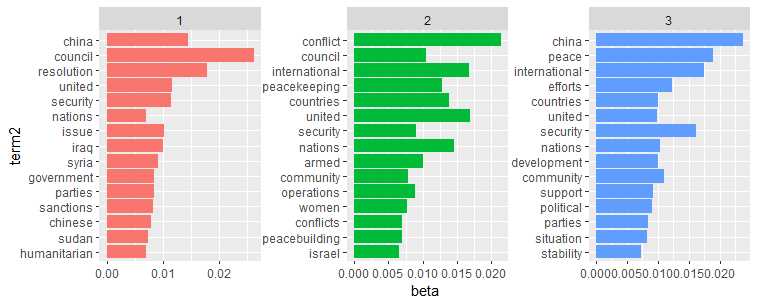
\includegraphics{Images/three topics.png} \\
\midrule
\endhead
Figure: Three-topic LDA model \\
\bottomrule
\end{longtable}

\hypertarget{conclusion}{%
\section{Conclusion}\label{conclusion}}

All in all we can say that the data by Schoenfeld et al. (2019) is very
rich and perfectly suitable for conducting text analysis.

\newpage

\hypertarget{references}{%
\section*{References}\label{references}}
\addcontentsline{toc}{section}{References}

\hypertarget{refs}{}
\begin{CSLReferences}{1}{0}
\leavevmode\vadjust pre{\hypertarget{ref-Loughran}{}}%
{``Documentation for the LoughranMcDonald\_MasterDictionary.''}
\url{https://www3.nd.edu/~mcdonald/Word_Lists_files/Documentation/Documentation_LoughranMcDonald_MasterDictionary.pdf}.

\leavevmode\vadjust pre{\hypertarget{ref-datacamp}{}}%
Dotson, Marc. n.d. {``Introduciton to Text Analysis in r.''} DataCamp.
\url{https://app.datacamp.com/learn/courses/introduction-to-text-analysis-in-r}.

\leavevmode\vadjust pre{\hypertarget{ref-textML}{}}%
Gavrilova, Yulia. 2020. {``Machine Learning \& Text Analysis.''}
Serokell. 2020.
\url{https://serokell.io/blog/machine-learning-text-analysis}.

\leavevmode\vadjust pre{\hypertarget{ref-grimmer2013}{}}%
Grimmer, Justin, and Brandon M Stewart. 2013. {``Text as Data: The
Promise and Pitfalls of Automatic Content Analysis Methods for Political
Texts.''} \emph{Political Analysis} 21 (3): 267--97.

\leavevmode\vadjust pre{\hypertarget{ref-GeneralInquirer}{}}%
Hall, William James. 2019. {``Harvard Iv-4 General Inquire
Dictionary.''} 2019.
\url{http://www.wjh.harvard.edu/~inquirer/homecat.htm}.

\leavevmode\vadjust pre{\hypertarget{ref-UNSC}{}}%
Schoenfeld, Mirco, Steffen Eckhard, Ronny Patz, Hilde van Meegdenburg,
and Antonio Pires. 2019. {``{The UN Security Council Debates}.''}
Harvard Dataverse. \url{https://doi.org/10.7910/DVN/KGVSYH}.

\leavevmode\vadjust pre{\hypertarget{ref-tidytext}{}}%
Silge, Julia, and David Robinson. 2017. \emph{Text Mining with r: A Tidy
Approach}. " O'Reilly Media, Inc.".
\url{https://www.tidytextmining.com/}.

\leavevmode\vadjust pre{\hypertarget{ref-wolfs}{}}%
Zhu, Zhiqun. 2020. {``Interpreting China's {`Wolf-Warrior
Diplomacy'}.''} \emph{The Diplomat} 15: 648--58.

\leavevmode\vadjust pre{\hypertarget{ref-ML2019}{}}%
Žižka, Jan, František Dařena, and Arnošt Svoboda. 2019. \emph{Text
Mining with Machine Learning: Principles and Techniques}. CRC Press.

\end{CSLReferences}

\hypertarget{appendix}{%
\section*{Appendix}\label{appendix}}
\addcontentsline{toc}{section}{Appendix}

\end{document}
